\section{Parameter Estimation using Optimization}
Initial parameters are found in the previous\fxnote{perhaps reff here}, however if the model is compared with reality\fxnote{figure or reff to earlier graph of this} it is evident that some further tuning of the parameters is needed. This can be solved using optimization, where (in this case) a Matlab script is given test data along with the model, and then given the task to fit the model output to the test data by adjusting one or more parameters in the model. In this case the model representation supplied to the script is a Simulink model, which can then be run by the script whenever needed and the script can modify the parameters to be adjusted. The process is iterative in most cases.

%Sense Tool is a Matlab toolbox and is utilized for the final tuning of model parameters. Sense Tool is given data from an initial value test of the Cubli hanging down like a pendulum, see \appref{impulseResponseAppendix}. Additionally some simulation must be supplied for the toolbox to test the parameters in each iteration. The simulation method used in this case is a Matlab Simulink model which is then run by Sense Tool when needed.
%Sense Tool is build with a Gauss-Newton Method implementation for solving the optimization problem leading to the parameter estimations. In the following a brief description of the principles behind this method is presented.

\subsection{The Optimization Problem}
The data provided is taken from an initial value test of the Cubli hanging down like a pendulum, see \appref{impulseResponseAppendix}. Furthermore the nonlinear model is used to accurately describe the oscillatory behavior of the pendulum. The model is modified, such that it describes the system as a regular pendulum without the dynamics of the reaction wheel, in order to match the test conditions under which the data was extracted\fxnote{Figure of the modified model is need here .. or reff}. In order to minimize the difference between the data points measured in test and the output of the model a function to describe such a relationship is needed. The performance function used to describe goodness of the fit, is a mean square error function.
%
\begin{flalign}
	\eq{\vec{P}(\vec{\theta})} {\frac{1}{mN}\sum_{k = 1}^{N} \left(\vec{y}(kT) - \vec{y_m}(kT, \vec{\theta})\right)^2 } &
\label{performanceFunction}
\end{flalign}
%
\hspace{6mm} Where:\\
\begin{tabular}{ p{1cm} l l l}
& \si{\vec{\theta}}   & is the parameter(s) to be adjusted                  & \\
& \si{N}              & is the degrees of freedom for each parameter        & \\
& \si{m}              & is the number of parameters to be adjusted          & \\
& \si{k}              & is the sample indexes, \si{k=1,\ 2,} ...\si{,\ N}   & \\
& \si{T}              & is the sampling time                                & \\
& \si{\vec{y}}        & is the test measurement output vector               & \\
& \si{\vec{y_m}}      & is the model output vector                          & \\
\end{tabular}

\fxnote{we need to figure out if [m is the number of parameters to be adjusted] is true - stated in where-list - in the documentation for Sense Tool m=2, why? Normally for MSE m=1}
The optimization problem is then defined as minimization of this performance function.

\subsection{Steepest Descent Method}
One way of solving the optimization problem is through use of the gradient. The gradient indicates in which direction the steepest descent or ascent is found in an infinitesimal surrounding of a given starting point.

For a function \si{f(x)} with a change in \si{x} of \si{\delta} the following can be obtained 
from the Taylor series.
%
\begin{flalign}
  f(x) + \Delta f(x) = f(\vec{x}+\vec{\delta}) &\approx f(x) + \vec{g}^T \vec{\delta} + \frac{1}{2} \vec{\delta}^T \vec{H}\vec{\delta} &
\label{taylorApproximation}
\end{flalign}
%
\hspace{6mm} Where:\\
\begin{tabular}{ p{1cm} l l l}
& \si{\vec{g}} 					    	   & is the gradient \si{\nabla f(x)}     & \\
& \si{\vec{H}} 					    	   & is the Hessian                       & \\
& \si{\vec{\delta}} 					   & is the change in \si{x}              & \\
\end{tabular}

%Then the change in \si{f(x)} as \si{||\vec{\delta}||_2 \rightarrow 0} can be approximated as follows.
%%
%\begin{flalign}
%  \Delta f(x) &\approx \vec{g}^T \vec{\delta} = ||\vec{g}||_2 \ ||\vec{\delta}||_2 \ cos \theta &
%\label{changeInF}
%\end{flalign}
%%
%\hspace{6mm} Where:\\
%\begin{tabular}{ p{1cm} l l l}
%& \si{\theta} 					    	   & is the angle between \si{\vec{g}} and \si{\vec{\delta}}     & \\
%\end{tabular}

In steepest descend method only the first order Taylor approximation is used, that is, the last term, \si{\frac{1}{2} \vec{\delta}^T \vec{H}\vec{\delta}} is discarded. If the derivative of the first order approximation, is set to zero, the following is obtained.
%
\begin{flalign}
  \frac{\partial}{\partial \vec{\delta}} \ f(\vec{x}+\vec{\delta}) &\approx \vec{g} = 0 &
\label{1stOrderTaylorApproximationParThetaEqZero}
\end{flalign}

That is, if the gradient of the function to be minimized is 0, a minimum or maximum exists as a candidate for a solution in this point. It follows that if standing in some point and taking the gradient in this point, then the gradient, \si{\vec{g}}, is the steepest ascend and the negative gradient, \si{-\vec{g}}, is the steepest descend. This only takes into account the immediate surroundings of the initially chosen point. One way of implementation is to set a step-size which decides how far in the \si{-\vec{g}} direction to go. The step-size can then be scaled in each itteration to avoid taking too large steps as shown in \figref{SteepestDescendLargeStep} and \figref{SteepestDescendSmallStep}.
%
\begin{minipage}{\linewidth}
	\begin{minipage}{0.45\linewidth}
		\begin{figure}[H]
			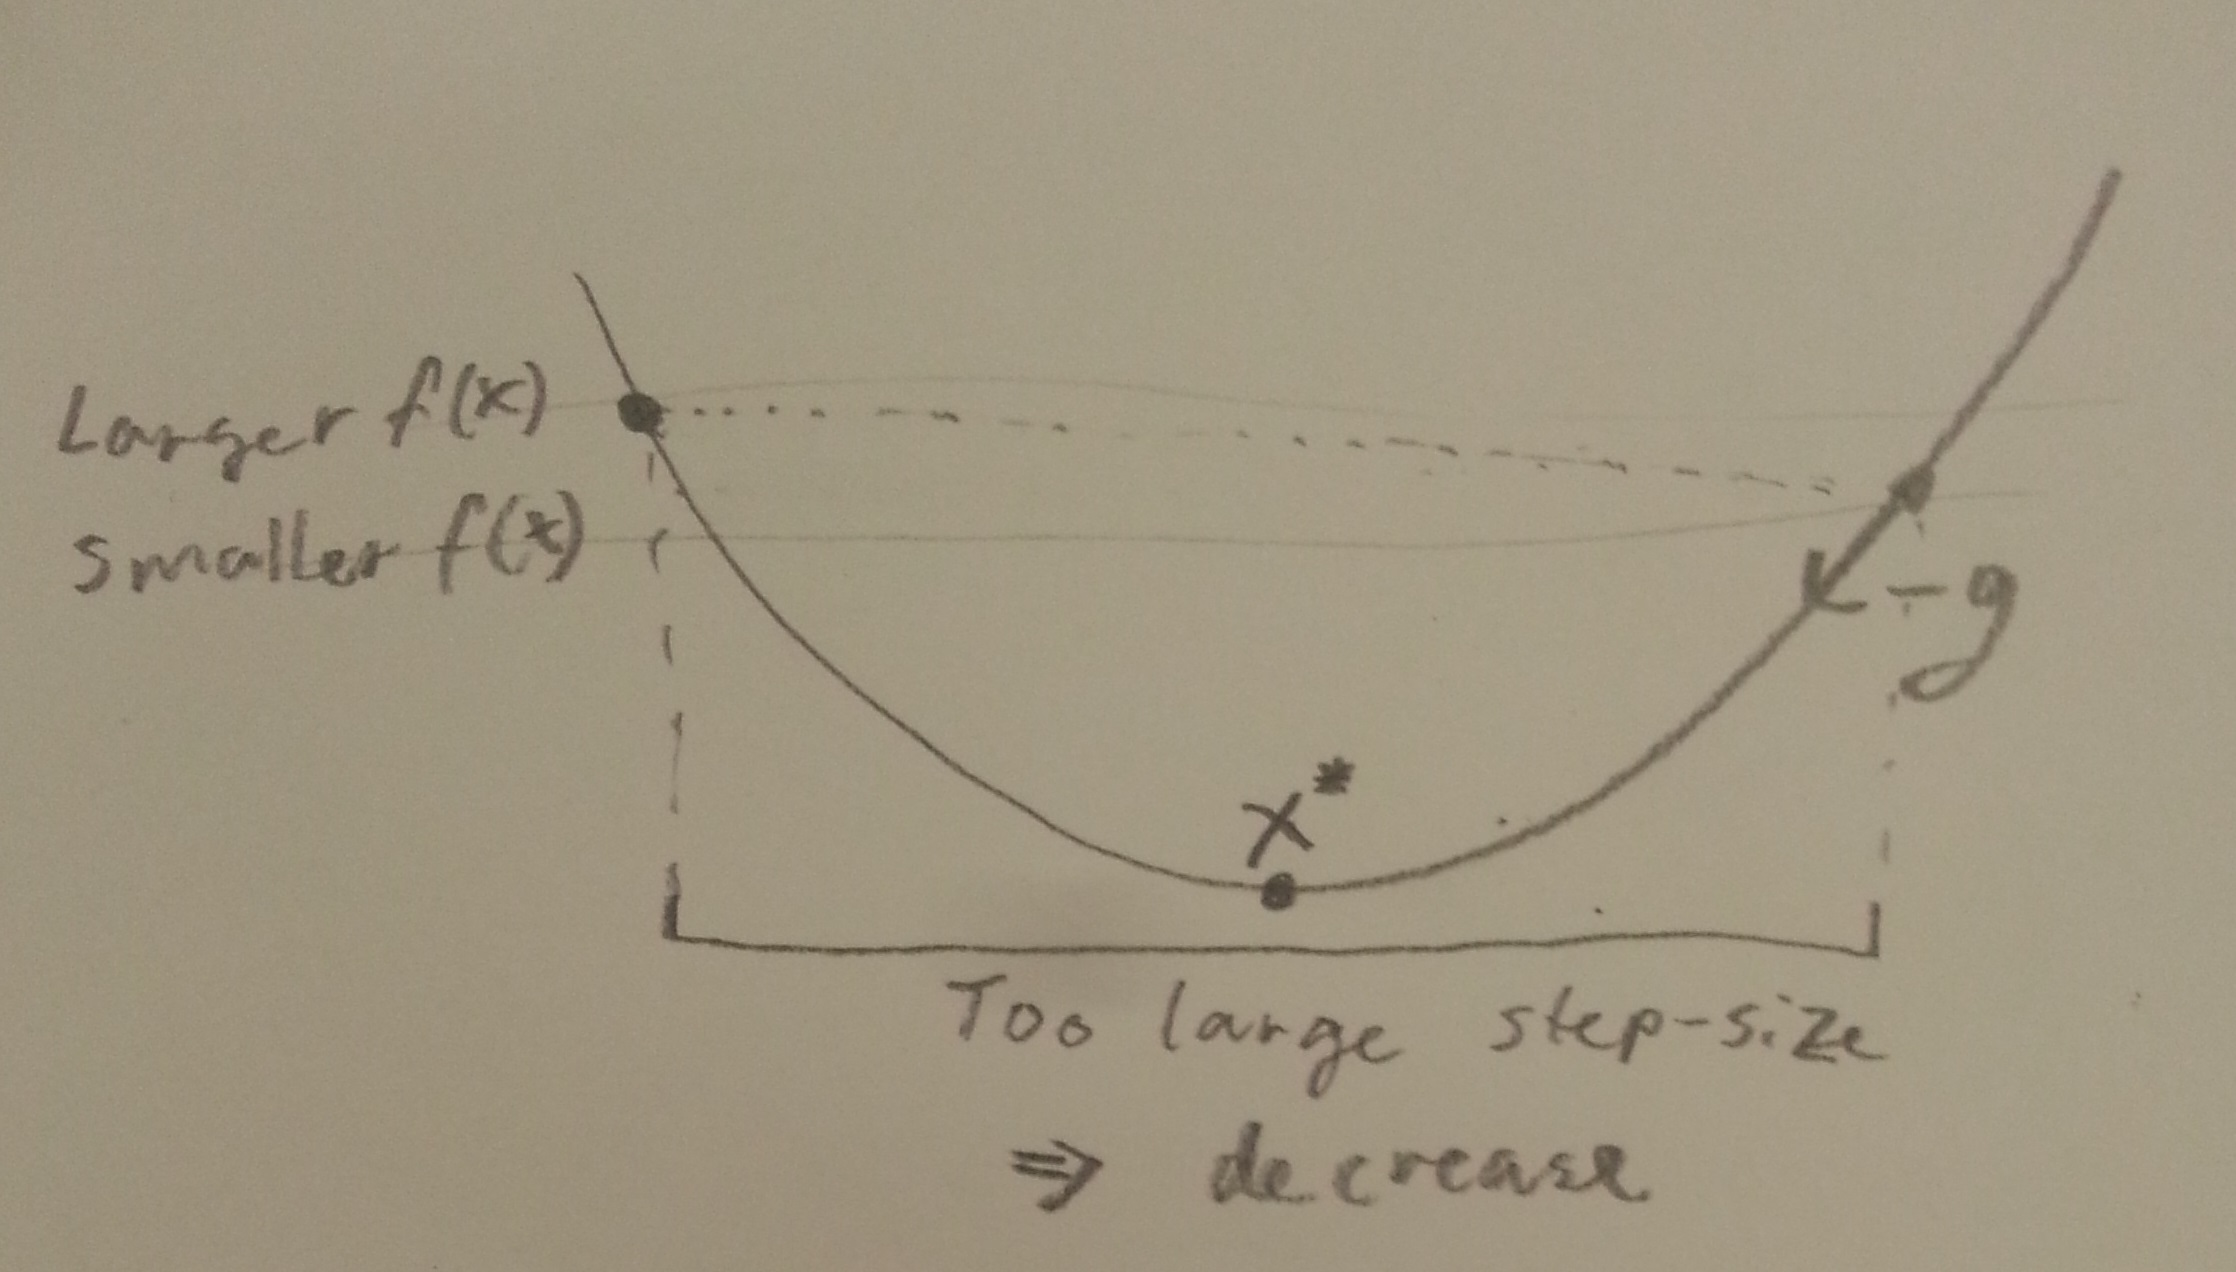
\includegraphics[scale=.09]{figures/SteepestDescendLargeStep}
			\centering
			\captionsetup{justification=centering}
			\vspace{-.55cm}
			\captionof{figure}{A too large step will cause the algorithm to step over the valley, resulting in a larger value of f(x) in the \si{-\vec{g}} direction}
			\label{SteepestDescendLargeStep}
		\end{figure}
	\end{minipage}
	\hspace{0.03\linewidth}
	\begin{minipage}{0.45\linewidth}
		\begin{figure}[H]
			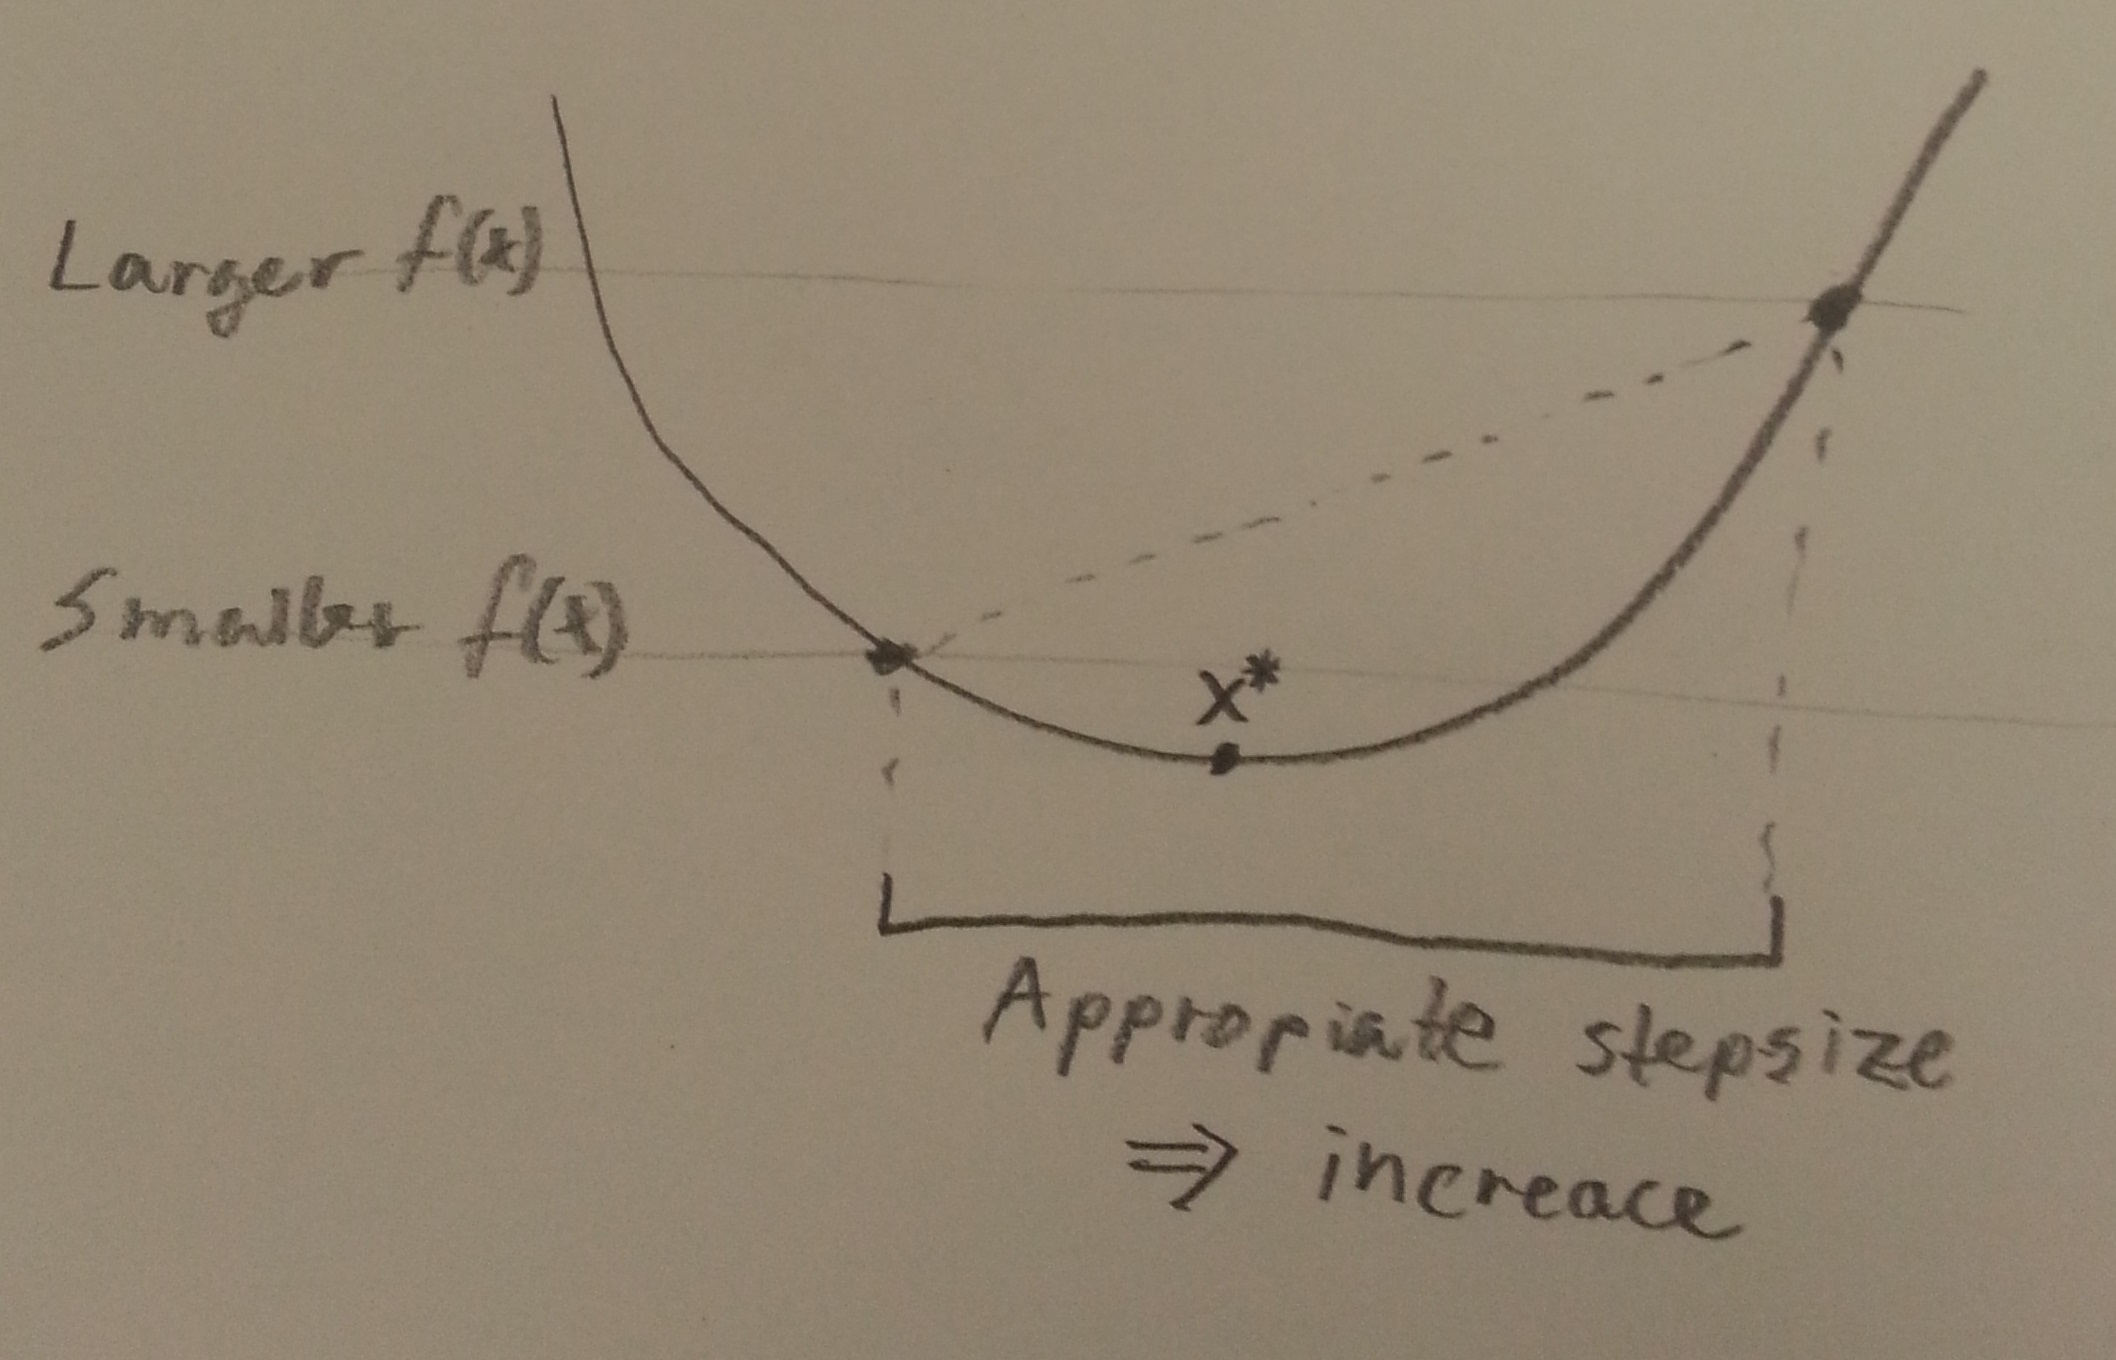
\includegraphics[scale=.084]{figures/SteepestDescendSmallStep}
			\centering
			\captionsetup{justification=centering}
			\captionof{figure}{By going back and choosing a smaller step, a smaller value for f(x) is obtained}
			\label{SteepestDescendSmallStep}
		\end{figure}
	\end{minipage}
\end{minipage}

The steepest descend method does find a minimum, however, it converges to the minimum rather slowly.

\subsection{Newton's Method}
An other approach is called Newton's Method is also rooted in the Taylor approximation, this however method however also uses the second order term of the approximation.
%
\begin{flalign}
  f(x) + \Delta f(x) = f(\vec{x}+\vec{\delta}) &\approx f(x) + \vec{g}^T \vec{\delta} + \frac{1}{2} \vec{\delta}^T \vec{H}\vec{\delta} &
\label{taylorApproximation2ndOrder}
\end{flalign}

In this case the derivative of the approximation is set to 0, and the following is obtained.
%
\begin{flalign}
  \frac{\partial}{\partial \vec{\delta}} \ f(\vec{x}+\vec{\delta}) &\approx \vec{g} + \frac{1}{2}\ \frac{\partial}{\partial \vec{\delta}}\ \vec{H}\vec{\delta}^2 &\\
  \frac{\partial}{\partial \vec{\delta}} \ f(\vec{x}+\vec{\delta}) &\approx \vec{g} + \vec{H}\vec{\delta} = 0 &
\label{2stOrderTaylorApproximationParThetaEqZero}
\end{flalign}

Using this to find an expression for the difference in \si{x}, \si{\vec{\delta}}, yields the following.
%
\begin{flalign}
  0 &= \vec{g} + \vec{H}\vec{\delta}  &\\
  \vec{\delta} &= -\vec{H}^{-1}\vec{g} &
\label{NewtonsMethod}
\end{flalign}

This expression can then be used to choose the value of \si{\vec{\delta}} such that \si{f(x)} is minimized.\fxnote{some visualization of how this works}

\subsection{Implementation of Newton's Method}
When implementing Newton's Method both the gradient and the Hessian of the performance function \eqref{performanceFunction} is needed\fxnote{Do we want the whole derivation of this?}.
%
\begin{flalign}
	\frac{\partial \vec{P}(\vec{\theta}) }{\partial \vec{\theta}} &= G(\vec{\theta}) = \frac{\partial}{\partial \vec{\theta}} \left( \frac{1}{mN}\sum_{k = 1}^{N} \left(\vec{y}(kT) - \vec{y_m}(kT, \vec{\theta})\right)^2 \right) &\\
  \eq{\vec{G}(\vec{\theta})} {- \frac{2}{mN}\sum_{k = 1}^{N} \left((\vec{y}(kT) - \vec{y_m}(kT, \vec{\theta})) \ \frac{\partial  \vec{y_m}(kT, \vec{\theta})}{\partial \vec{\theta}} \right) } &
\label{gradientOfPerformanceFunction}
\end{flalign}

Since the Matlab implementation uses a Simulink model the problematic part of \eqref{gradientOfPerformanceFunction} is the derivative of the model with respect to the model parameters, \si{\frac{\partial  \vec{y_m}(kT, \vec{\theta})}{\partial \vec{\theta}}}. To solve this problem a numerical differentiation of the model is applied as shown in \autoref{AlgorithmForNummericalDiff}.

\begin{lstlisting}[ language = Matlab,
                    caption  = {Algorithm for numerical differentiation of the simulated model},
                    label    = AlgorithmForNummericalDiff ]

  %small deviation from parameters, J_f and B_f, is set
  p = 0.001;
  
  %calculating the deviation
  deltaJ_f = p*J_f; deltaB_f = p*B_f;
  
  %saving the old parameters:
  J_f_old = J_f; B_f_old = B_f;
  
  %setting deviating parameters ready for simulation
  J_f = deltaJ_f;
  
  %running the simulation again, now with deviation in J_f
  sim('CubliSenseToolSim.slx');
  
  %storring the result of the simulation
  deltaYmJf = simOut;
  
  %setting deviating parameters ready for simulation
  B_f = deltaB_f; J_f = J_f_old; %<--restoring J_f
  
  %running the simulation again, now with deviation in B_f
  sim('CubliSenseToolSim.slx');
  
  %storring the result of the simulation
  deltaYmBf = simOut;
  
  %restoring the parameters to their original value
  B_f = B_f_old;
  
  %calculating the derivatives of the model
  YmDiffBf = ( deltaYmBf - Ym )/ p;
  YmDiffJf = ( deltaYmJf - Ym )/ p;
\end{lstlisting}
